%%!Mode:: "Tex:UTF-8"
\chapter{分散式事件激发采样下带马氏切换的非线性随机耦合网络同步问题}\label{chapternonline}
    目前, 复杂网络同步问题已经得到研究者广泛研究. 早些时候的网络同步问题的理论成果主要是建立在固定耦合拓扑的假设之上, 即网络节点间的耦合关系只有一种模式. 后来有研究者发现, 在实际应用中网络节点间的关系并不是一成不变的. 例如在企业关系网中, 企业与企业之间某时期是竞争关系, 但在某时期会转为合作关系. 显然, 变化的拓扑结构更加适应于实际的网络模型. 研究者们提出, 通过引入马氏链来模拟网络拓扑结构在不同外环境中的切换过程.

    本文在前人的基础上, 继续探讨具有切换拓扑结构的复杂网络同步问题.
    节点间的线性耦合是较为简单的耦合方式, 对于大规模节点的网络, 节点间的耦合关系往往不能够直接观测得到, 而是观测到其经过非线性函数映射后的结果. 因此研究非线性耦合的结构更符合实际网络环境且更具有挑战性. 特别是在保密通讯方面, 线性的耦合结构比较容易受到黑客的攻击, 不利于通讯安全. 将信号通过非线性转换后再传输能够极大地提高了信息传输的安全性.

    很多现实中的网络很难达到同步或者同步时间较长, 因此需要引进控制方法促进网络快速到达同步. 控制方法根据采样时间是否连续可以分为连续采样控制和非连续采样控制, 其中非连续采样控制方法有周期间歇控制、脉冲控制、以及基于事件激发采样控制. 事件激发采样控制策略的基本思想是网络节点间的信息传输只发生在事件激发时刻, 而该时刻由只依赖于节点自身状态信息以及邻居节点上一次更新的状态信息的激发规则决定. 当激发规则满足时, 事件就会被激发, 此时采样行为发生, 相应的控制器发生更新. 基于事件激发采样不仅可以减少控制器的更新频率, 同时还可以减少节点间的通讯负荷. 根据节点是否具有一致的激发时刻, 可将事件激发采样分为分散式和集中式两种. 本章节采用的是分散式事件激发采样的控制策略去研究带有马氏切换非线性耦合复杂网络的同步问题.

    %在实际应用中, 由于系统可能会受到不可以预知的外在因素干扰, 复杂网络节点间的耦合关系并不是一成不变的, 节点与节点之间时而存在耦合关系, 时而中断耦合关系. 例如, 设备之间的通讯会受到电磁干扰、温度干扰、湿度干扰、声波干扰、振动干扰和射频辐射干扰等等, 从而会导致设备间的信号传输随时都有可能发生中断. 因此研究随机发生耦合复杂网络更具有实际应用. 目前, 有一部分研究者已经对随机发生耦合网络展开了相关的研究, 并取得了一些成果. 例如Yang\upcite{X18}和Baumeister\upcite{M19}等人分别研究了随机发生耦合神经网络的同步问题, 并给出了有效的同步判据. 然而这些作者一般考虑都是线性的耦合关系, 事实上, 网络节点之间的状态信息有时候很难观察到线性变量的值, 而只能观测到它的非线性函数的值. 故非线性耦合网络更有研究的必要. 除此之外, 很多现实中的网络很难到达同步或者同步时间耗时较长, 因此需要引进控制方法驱使网络快速到达同步\upcite{Lu9,Turci11,Jin12,Turci13,Li15,pwang30,ptang31,22,nonl-asym}. 尽管这些文献都提出了各种各样的控制方法, 但是它们都有一个共同的特点, 那就是控制都是实时更新的, 控制器频繁更新会加大能量损耗和通讯负荷. 理想的情况应该是根据网络系统的情况, 按照需要来更新控制器. 例如在军训时候, 教官为了使得学生的步伐达到同步, 会根据队伍的情况发出口令进行控制, 而不是教官一直不停地发出口令. 基于事件激发的控制策略正是解决控制器频繁更新的问题, 该策略是根据网络系统节点间关系、以及节点自身与同步目标之间的关系构造一个激发规则, 当激发规则满足时, 事件就会被激发, 相应的控制器发生更新. 这不仅可以减少控制器的更新频率, 同时可以见到节点间的通讯负荷. 本文就是利用事件激发的策略研究带有马氏切换非线性耦合复杂网络同步的问题.

\section{分散式事件激发采样的网络模型}\label{csnp:sec:moper}
        分散式事件激发采样的特点是每个节点都有自己的激发规则, 某节点的激发并不会引起其他邻居节点的激发, 但会将该激发时刻的采样信息转告给邻居节点使其更新激发规则. 本章节利用基于分散式事件激发采样的牵制控制方法研究带有马氏切换的随机发生非线性耦合复杂网络同步问题. 网络的随机性不仅体现在耦合模式是随机切换的, 同时还体现在随机发生的耦合以及随机耦合强度. 其网络模型如下:
        %在网络控制理论中, 根据控制节点的数量可以将控制方法分为全局控制和牵制控制(局部控制). 牵制控制主要思想是通过控制较少的节点, 然后通过网络节点间的联系来传输控制信号以实现网络同步. 相比于全局控制, 牵制控制能够节省控制成本. 有时候只需控制一个节点就可以实现了网络同步. 一般在控制节点的选择上偏向于具有较大度的节点. 本节将牵制控制方法和事件激发策略相结合, 研究带有马氏切换的随机发生非线性耦合复杂网络同步问题. 网络模型如下:
        \begin{align}\label{sys:init1}
        \nonumber\dot{x}_{i}(t)&=f(x_{i}(t))-\theta(t)\rho(t)\sum^N_{j=1}l_{ij}(r_{t})\Gamma[h(x_{j}(t_{k}^{i}))-h(x_{i}(t_{k}^{i}))]+u_i(t), \\
        &\quad t_{k}^i\leq t< t_{k+1}^i, i = 1,\cdots,N,
        \end{align}
        其中$\theta(t)$是伯努利随机变量, 满足$P(\theta(t)=1)=\theta\in(0,1)$, 它描述网络系统随机发生的耦合;
        $\rho(t)$是随机耦合强度, 其$\mathrm{E}[\rho(t)]=c>0, \mathrm{Var}(\rho(t))<\infty$. 这里假设$\sigma(t), \theta(t)$和$\rho(t)$是相互独立的; $h( x_{i}(t))=(h_{1}(x_{i}^{1}(t)),h_{2}(x_{i}^{2}(t)),\cdots,h_{n}(x_{i}^{n}(t)))^{\top}\in R^{n}$是非线性耦合函数;
        $t_k^i$是第$i$个节点第$k$次事件激发的时刻.
        控制输入$u_i(t)$的定义如下:
        \begin{align}\label{nonlinearcontrol}
            u_i(t)=-\tau \rho(t)d_{i}(r_{t})\Gamma[h(x_{i}(t_{k}^{i}))-h(s(t_{k}^{i}))],
        \end{align}
        这里$\tau\rho(t)$是控制增益; $d_{i}(r_{t})=I_{\{i\in \mathcal D(r_{t})\}}$是牵制节点集$\mathcal D(r_{t})\subset \{1,2,\cdots,N\}$上的示性函数, 即, 如果$i\in \mathcal D(r_{t})$, 则$I_{\{i\in \mathcal D(r_{t})\}}=1$, 否则$I_{\{i\in \mathcal D(r_{t})\}}=0$; $s(t)$ 是孤立节点动力学$\dot{s}(t)=f(s(t))$的轨道, 即同步的目标轨道.
        \begin{rem}
            该模型与 \eqref{eventcontrolnetwork} 的不同之处是每个节点都具有自己的激发时刻, 且增加了非线性耦合、随机发生的耦合、以及随机耦合强度. 它更加符合实际生活中的系统, 具有更广泛的应用价值.
        \end{rem}

\section{分散式事件激发采样的复杂网络同步分析}
    本节主要探索在连续时间监控和离散时间监控下, 网络系统 \eqref{sys:init1} 能够达到同步的条件. 通过构造合适的事件激发规则, 结合稳定性理论, 推导出在两种情形下的同步判据. 在给出结论之前, 先给出必要的引理.
    \begin{lem}\label{lem:5}
            设矩阵$Q\in R^{n \times n}$满足$q_{ij}=q_{ji}$, $q_{ii} =-\sum_{j=1,i \neq j}^n q_{ij}(i,j=1,2,\ldots,n)$, 则对任意向量$u=(u_1,u_2,\ldots,u_n)^\top$, $v=(v_1,v_2,\ldots,v_n)^\top$, 有
            $$u^\top Qv=\sum_{i=1}^n\sum_{j=1}^n u_i q_{ij} v_j=-\sum_{j>i}q_{ij}(u_i-u_j)(v_i-v_j).$$
    \end{lem}
    \begin{lem}[Gronwall—Bellman不等式]\label{lem:6}{\rm\upcite{Gronwall,Bellman}}
        设$\varphi(t), \alpha(t), \beta(t)$是区间$[a,b]$上的连续函数.

       情形$1:$ 如果$\varphi(t)$在区间$[a,b]$上非负可微, 且对任意$t\in [a,b]$, 有
            $$\dot{\varphi}(t)\geq \alpha(t)\varphi(t)+\beta(t).$$
       那么
            $$\varphi(t)\geq\varphi(a)e^{\int^{t}_{a}\alpha(s)ds}+\int^{t}_{a}\alpha(s)\beta(s)e^{\int^{t}_{s}\beta(u)du}ds.$$

       情形$2:$ 如果$\beta(t)$在区间$[a,b]$上非负可积, 且对任意$t\in [a,b]$, 有
            $$\varphi(t)\leq \alpha(t)+\int^{t}_{a}\beta(s)\varphi(s)ds.$$
         那么
            $$\varphi(t)\leq \alpha(t)+\int^{t}_{a}\alpha(s)\beta(s)e^{\int^{t}_{s}\beta(u)du}ds.$$
    \end{lem}
    由于非线性耦合的结构形式众多, 并且及其复杂, 这里我们仅讨论符合以下假设的非线性函数类.
    \begin{hyp}\label{ass}
        假设存在正数$\alpha_{k}$, $\beta_{k}(k=1,2,\cdots,n)$, 使得对任意$x,y\in R$, 有
                $$\alpha_{k}\leq\frac{h_{k}(x)-h_{k}(y)}{x-y}\leq\beta_{k}.$$
    \end{hyp}
    \begin{rem}
        假设 \ref{ass} 是比较常见的, 只要函数满足一阶导数有界并且导数值为正数即可, 例如反正切函数就可以满足.
    \end{rem}
    记$e_{i}(t)=x_{i}(t)-s(t)(i=1,2,\cdots,N)$为节点$i$的同步误差. 为了讨论方便, 引入下述记号:
        %\begin{flalign}
        %\begin{split}
        \begin{eqnarray*}
        &&f(e_{i}(t))=f(x_{i}(t))-f(s(t)),\\
        &&h(e_{i}(t))=h(x_{i}(t))-h(s(t)),\\
        &&e(t)=(e^\top_{1}(t),e^\top_{2}(t),\cdots,e^\top_{N}(t))^\top,\\
        &&f(e(t))=(f^\top(e_{1}(t)),f^\top(e_{2}(t)),\cdots,f^\top(e_{N}(t)))^\top,\\
        &&h(e(t))=(h^\top(e_{1}(t)),h^\top(e_{2}(t)),\cdots,h^\top(e_{N}(t)))^\top,\\
        &&D(r_{t})=\text{diag}\{d_{1}(r_{t}),d_{2}(r_{t}),\cdots,d_{N}(r_{t})\}.
        %\end{split}&
        %\end{flalign}
        \end{eqnarray*}
       于是网络系统 \eqref{sys:init1} 可以写成误差系统的形式:
        \begin{align}\label{sys:all}
        \dot{e}(t)=f(e(t))-\theta(t)\rho(t)[L(r_{t})\otimes\Gamma]h(e(t))-\tau \rho(t)[D(r_{t})\otimes\Gamma] h(e(t))+\rho(t)\tilde{e}(t),
        \end{align}
       其中$\tilde{e}(t)=(\tilde{e}^\top_{1}(t),\tilde{e}^\top_{2}(t),\cdots,\tilde{e}^\top_{N}(t))^\top$ 是系统测量误差, 其分量定义为如下:
        \begin{align*}
        \nonumber \tilde{e}_{i}(t)=&\theta(t)\sum^{N}_{j=1}l_{ij}(r_{t})\Gamma[h(x_{j}(t))-h(x_{j}(t_{k}^{i}))]\\
        &-\tau d_{i}(r_{t})[h(x_{i}(t))-h(x_{i}(t_{k}^{i}))+h(s(t_{k}^{i}))-h(s(t))].
        \end{align*}
\subsection{连续监控激发规则}
    在连续监控情形下, 监控器实时地收集节点$x_i(t), x_j(t)$和$s(t)$的状态信息, 事件激发规则根据收集到的节点状态信息判断此时是否满足激发条件. 如果关于某个节点$i$ 的激发规则满足, 则关于节点$i$的事件就被激发, 从而获得新的事件激发时刻$t^{i}_{k+1}$. 与此同时, 节点$i$更新自身状态和控制器状态, 并且发送$t^i_{k_i(t)}$时刻的状态信息给邻居节点, 这里$k_{i}(t)=$argmax$_{k^{'}}\{t^{i}_{k^{'}}\leq t\}$. 于是邻居节点更新$t^{i}_{k}$时的状态信息为$t^{i}_{k+1}$ 时的状态信息, 但关于邻居节点的事件不会被激发直到属于邻居节点的激发条件满足. 具体流程见\autoref{cflowchart}.
    \begin{figure}[!htp]
    \setlength{\abovecaptionskip}{-1cm}
     \begin{center}
           {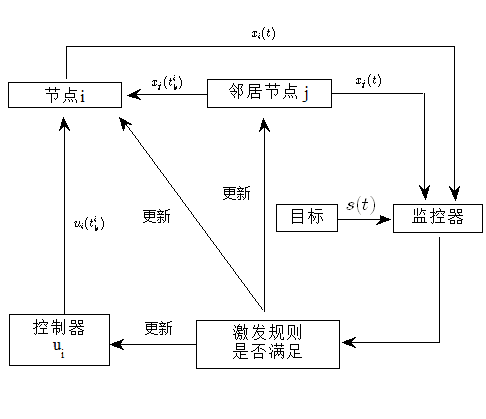
\includegraphics[width=3.2in]{nonlinear/flowchartcon1.png}}
     \end{center}
  \caption{连续监控下事件激发牵制控制流程图}\label{cflowchart}
    \end{figure}

    下面给出两种不同误差上界的激发规则:

           情形a: 基于同步误差上界的连续监控事件激发规则(简称为CRS激发规则):
            \begin{equation}\label{crule:1}
            t^{i}_{k+1}=\max\left\{t\geq t^{i}_{k}: \|\tilde{e}_{i}(t)\| \leq\omega \| e_{i}(t)\|\right\}
            \end{equation}

            情形b: 基于指数函数上界的连续监控事件激发规则(简称为CRE激发规则):
            \begin{equation}\label{crule:2}
             t^{i}_{k+1}=\max\left\{t\geq t^{i}_{k}: \|\tilde{e}_{i}(t)\| \leq ae^{-bt}\right\}
             \end{equation}
           其中$\omega=\frac{2\xi\underline{\varepsilon}-\delta\bar{\varepsilon}}{2c\bar{\varepsilon}}$, $0<\delta\leq\frac{2\xi\underline{\varepsilon}}{\bar{\varepsilon}}$, $a>0$, $b>0$,
              $\underline{\varepsilon}=\min_{v}\{\lambda_{min}(P(v))\cdot\lambda_{min}(G)\}$, $\bar{\varepsilon}=\max_{v}\{\lambda_{max}(P(v))\cdot\lambda_{max}(G)\}$.

            网络系统激发的具体算法如下:
            \begin{algo}[连续监控事件激发算法]\label{algo1}~~

            $1)$ 当$k=0$时, 初始化$t^i_k=0$;

            $2)$ 当$t\geq t^i_k$时, 监控器实时收集节点$x_i(t),x_j(t)$, $s(t)$的状态信息;

            $3)$ 如果$\|\tilde{e}_{i}(t)\|>\omega \| e_{i}(t)\|($或者 $\|\tilde{e}_{i}(t)\| > ae^{-bt})$, 则事件被激发, 最新的激发时刻$t^i_{k+1}=t$, 返回$2)$;

            $4)$ 当$t=t^i_{k+1}$时, 节点$i$以及它的邻居节点和控制器将会更新状态信息, 即用$t_{k+1}^i$时刻状态信息替换$t^i_{k}$时刻的状态信息, 返回$2)$.
             \end{algo}

        下面给出连续监控情形下的同步判定定理.
        \begin{thm}\label{themcon}
            如果假设 $\ref{ass}$ 成立, $f(\cdot)$属于$QUAD(G,\Delta,\xi)$, 并且存在正定对角阵$P(u)=\mathrm{diag}\{p_{1}(u),\cdots p_{N}(u)\}$, $u\in S$, 使得对任意$u\in S$, 有
            \begin{align}\label{nonthm:1}
            \bar{\delta}P(u)\otimes G-c\theta\underline{\alpha} P(u)L(u)\otimes G\Gamma
            -c\tau\underline{\alpha} P(u)D(u)\otimes G\Gamma+\frac{1}{2}\sum_{v=1}^{m}q_{uv}P(v)\otimes G\leq 0,
            \end{align}
            其中$\bar{\delta}=\max_{k}\{\delta_k \}$, $\underline{\alpha}=\min_{k}\{\alpha_{k}\}$.
            那么, 基于$\mathrm{CRS}$激发规则或者$\mathrm{CRE}$激发规则, 按照算法 $\ref{algo1}$, 网络系统 \eqref{sys:init1} 可以实现均方指数同步.
        \end{thm}
        \begin{proof}
        在$r(t)=u\in S$时, 定义随机Lyapunov—Krasovskii函数$V(t)$如下:
        \begin{equation*}
            V(t)=\frac{1}{2}e^{\top}(t)[P(u)\otimes G]e(t).
        \end{equation*}
        记$\mathcal{L}$是弱无穷小生成元算子. 根据\autoref{lem:1} 和式 \eqref{sys:all} 以及$QUAD$条件, 有
            \begin{align}\label{diff:V}
            \nonumber \mathrm{E}\mathcal{L}V(t)&=\mathrm{E}\bigg\{e^{\top}(t)[P(u)\otimes G]\Big [F(e(t))-I\otimes\Delta e(t)+I\otimes\Delta e(t)-c\theta \left[L(u)\otimes\Gamma\right] H(e(t))\\
            \nonumber &\quad-c\tau[D(u)\otimes\Gamma] H(e(t))+c\tilde{e}(t)\Big]+\frac{1}{2}\sum_{v}q_{uv}e^\top(t)\left[P(v)\otimes G\right]e(t)\bigg\}\\
            \nonumber &\leq \mathrm{E}\bigg\{(\bar{\delta}-\xi)e^\top(t)[P(u)\otimes G]e(t)-c\theta e^{\top}(t)[P(u)L(u)\otimes G\Gamma] H(e(t))\\
            \nonumber &\quad-c\tau e^{\top}(t)[P(u)D(u)\otimes G\Gamma]H(e(t))+ce^{\top}(t)[P(u)\otimes G]\tilde{e}(t)\\
            &\quad+\frac{1}{2}\sum_{v}q_{uv}e^{\top}(t)\left[P(u)\otimes G\right]e(t)\bigg\}
            \end{align}
        下面处理上式中含有非线性的项, 根据\autoref{ass} 和\autoref{lem:5}, 可得
            \begin{align}\label{equ:2}
            \nonumber&\quad-\mathrm{E}\Big\{e^{\top}(t)[P(u)L(u)\otimes G\Gamma]H(e(t))\Big\}\\
            &=-\mathrm{E}\bigg\{\sum^{N}_{i=1}\sum^{N}_{j=1}e^{\top}_{i}(t)p_i(u)l_{ij}(u)G\Gamma h(e_{j}(t))\bigg\}\\
            \nonumber &=-\mathrm{E}\bigg\{\sum^{N}_{i=1}\sum^{N}_{j=1}p_i(u)l_{ij}(u)\sum^{n}_{k=1}e^{k}_{i}(t)g_{k}\gamma_{k}h_{k}(e^{k}_{j}(t))\bigg\}\\
            \nonumber &=-\mathrm{E}\bigg\{\sum^{n}_{k=1}g_{k}\gamma_{k}\sum^{N}_{i=1}\sum^{N}_{j=1}p_i(u)l_{ij}(u)e^{k}_{i}(t)h_{k}(e^{k}_{j}(t))\bigg\}\\
            \nonumber &=\mathrm{E}\bigg\{\sum^{n}_{k=1}p_{k}\gamma_{k}\sum_{j>i}p_i(u)l_{ij}(u)(e^{k}_{i}(t)-e^{k}_{j}(t))(h_{k}(e^{k}_{i}(t))-h_{k}(e^{k}_{j}(t)))\bigg\}\\
            \nonumber &\leq\underline{\alpha}\mathrm{E}\bigg\{\sum^{n}_{k=1}g_{k}\gamma_{k}\sum_{j>i}p_i(u)l_{ij}(u)(e^{k}_{i}(t)-e^{k}_{j}(t))^2\bigg\}\\
             &=-\underline{\alpha}\mathrm{E}\Big\{ e^{\top}(t)[P(u)L(u)\otimes G\Gamma]e(t)\Big\}.
            \end{align}
        利用类似的方法可得如下关系式:
            \begin{align}\label{equ:3}
            -\mathrm{E}\Big\{e^{\top}(t)[P(u)D(u)\otimes G\Gamma]H(e(t))\Big\}\leq-\underline{\alpha} \mathrm{E}\Big\{e^{\top}(t)[P(u)D(u)\otimes G\Gamma]e(t)\Big\}.
            \end{align}
        对于式 \eqref{diff:V} 中含有系统测量误差的项, 通过运用\autoref{lem:2} 和\autoref{lem_leq}, 可得
            \begin{align}\label{equ:4}
            \nonumber \mathrm{E}\Big\{e^{\top}(t)[P(u)\otimes G]\tilde{e}(t)\Big\}&\leq \mathrm{E}\Big\{\frac{\mu}{2}e^{\top}(t)[P(u)\otimes G]^2e(t)+\frac{1}{2\mu}\tilde{e}^{\top}(t)\tilde{e}(t)\Big\}\\
            &\leq \mathrm{E}\Big\{\frac{\mu\bar{\varepsilon}^2}{2}e^{\top}(t)e(t)+\frac{1}{2\mu}\tilde{e}^{\top}(t)\tilde{e}(t)\Big\},
            \end{align}
            其中$\mu$是正数. 将式 \eqref{equ:2}$-$\eqref{equ:4} 代入式 \eqref{diff:V}, 并结合式 \eqref{nonthm:1} 可得
            \begin{align}\label{equ:5}
            \nonumber \mathrm{E}\mathcal{L}V(t)&\leq \mathrm{E}\Big\{e^{\top}(t)\Big[\bar{\delta}P(u)\otimes G-c\theta\underline{\alpha} P(u)L(u)\otimes G\Gamma\\
            \nonumber &\quad-c\tau\underline{\alpha} P(u)D(u)\otimes G\Gamma+\frac{1}{2}\sum_{v=1}^{m}q_{uv}P(v)\otimes G\Big]e(t)\\
            \nonumber &\quad+(\frac{c\mu\bar{\varepsilon}^2}{2}+\frac{\delta\bar{\varepsilon}}{2}-\xi\underline{\varepsilon}) e^{\top}(t)e(t)
            +\frac{1}{2\mu}\tilde{e}^{\top}(t)\tilde{e}(t)-\frac{\delta\bar{\varepsilon}}{2}e^{\top}(t)e(t)\Big\}\\
            &\leq \mathrm{E}\Big\{(\frac{c\bar{\varepsilon}^2\mu}{2}-c\bar{\varepsilon}\omega)e^\top(t)e(t)+\frac{c\bar{\varepsilon}}{2\omega}\tilde{e}^{\top}(t)\tilde{e}(t)\Big\}
            -\delta EV(t,e(t)).
            \end{align}

            情形a: 当选用CRS激发规则时, 此时选择常数$\delta$使得$0<\delta\leq\frac{2\xi\underline{\varepsilon}}{\bar{\varepsilon}}$ 即可. 根据激发条件式 \eqref{crule:1} 可得
            \begin{align}\label{equ:18}
                \mathrm{E}\tilde{e}^{\top}(t)\tilde{e}(t)\leq\omega^2\mathrm{E}e^\top(t)e(t).
            \end{align}
            由于式 \eqref{equ:5} 对任意$\mu>0$都成立, 因此可取$\mu=\frac{\omega}{\bar{\varepsilon}}$并将其代入式 \eqref{equ:5}, 结合式 \eqref{equ:18}, 可得
            \begin{align*}
                \mathrm{E}\mathcal{L}V(t)\leq -\delta \mathrm{E}V(t).
            \end{align*}
            根据比较原理可得
            \begin{align*}
            \mathrm{E}V(t)\leq \mathrm{E}V(0)e^{-\delta t}.
            \end{align*}
            因此
            \begin{align*}
             \mathrm{E}\| x_{i}(t)-s(t)\|^2&\leq\frac{2}{\underline{\varepsilon}}\mathrm{E}V(0)e^{-\delta t},\quad i=1,2,\cdots,N.
            \end{align*}
            所以在CRS激发规则下, 网络系统 \eqref{sys:init1} 可以达到均方指数同步.

        情形b: 当选用CRE激发规则时, 根据激发条件式 \eqref{crule:2} 可得
            \begin{align}\label{equwan}
                \mathrm{E}\tilde{e}^{\top}(t)\tilde{e}(t)\leq Na^2e^{-2bt}.
            \end{align}
        因为式 \eqref{equ:5} 对任意$\mu>0$成立, 故取$\mu=\frac{2\omega}{\bar{\varepsilon}}$并代入式 \eqref{equ:5}, 结合式 \eqref{equwan}, 可得
            \begin{align*}
            \mathrm{E}\mathcal{L}V(t)
            \leq \frac{Nca^2\bar{\varepsilon}}{2\omega}e^{-2bt} -\delta \mathrm{E}V(t).
            \end{align*}
        求解上式相对应的微分方程并利用比较原理可得
            \begin{align*}
            \mathrm{E}V(t,e(t))&\leq\frac{Nca^2\bar{\varepsilon}}{2\omega(-2b+\delta)}\Big[e^{(-2b+\delta)t}-1\Big]e^{-\delta t}+ \mathrm{E}V(0,e(0))e^{-\delta t}
            =\pi e^{-\delta t},
            \end{align*}
        其中$\pi=\mathrm{E}V(0,e(0))+\frac{Nca^2\bar{\varepsilon}}{2\omega(-2b+\delta)}(e^{(-2b+\delta)t}-1)$. 根据$V(t)$的定义可得
             \begin{align*}
             \mathrm{E}\| x_{i}(t)-s(t)\|^2\leq\frac{2\pi}{\underline{\varepsilon}}e^{-\delta t},\quad i=1,2,\cdots,N.
            \end{align*}
           因此在CRE激发规则下, 网络系统 \eqref{sys:init1} 可以达到均方指数同步.
        \end{proof}
        \begin{rem}
           %System measurement error is controlled by synchronization error based CRS. It can adjust automatically synchronous speed and triggered frequency according to the synchronization error. Hence CRS costs less time than CRE in achieving synchronization. The advantage of CRE is that we can adjust synchronous speed and triggered frequency as required. In practical application, when the signal transmission costs a lot of energy, we can use CRE and select larger $a$ and smaller $b$ to reduce the triggered frequency. When we hope a system to achieve synchronization as soon as possible, CRS is a good choice.
           CRS激发规则中的系统测量误差被同步误差控制, 其系数$\omega$是由系统决定的, 不可以被修改. 而CSE激发规则中的系统测量误差被指数函数控制, 激发规则中的参数 $a$和$b$可以根据所需的同步速度和激发频率进行选择. 一般上, CRS激发规则的同步速度会比CRE激发规则快, 但是CRS激发规则的激发频率会高于CRE激发规则. 高激发频率会引起系统间的数据频繁更新, 因此CRS激发规则比CRE激发规则有更大的计算负荷. 至于监控成本方面, 两种激发规则花费的成本是一样的.
        \end{rem}

\subsection{离散监控激发规则}

        连续监控激发规则不仅需要实时监控节点的变化情况, 同时激发规则的信息也需要实时地更新. 因此连续监控会花费较高的监控成本和通讯负荷. 为了较少监控成本和通讯负荷, 这一节研究采用离散监控模式. 不同于连续监控激发策略, 在离散监控激发策略中, 节点的状态信息只在$t=t^i_k$ 时刻时监控. 然后根据最新监控得到的状态信息进行预测下一次事件激发的间隔$\pi_k^i$来确定下一次激发时刻. 当时间达到预测的激发时刻, 即$t=t_k+\pi_k^i$时, 关于节点$i$的事件就被激发, 新的激发时刻$t^i_{k+1}$ 被确定. 此时, 监控器记录该时刻的状态信息发送至控制器和各邻居节点. 同时节点$i$和其邻居节点重新预测下一次激发间隔. 详见\autoref{flowchart} 预测激发过程图.
        \begin{figure}[!htp]
        \setlength{\abovecaptionskip}{-1cm}
        \begin{center}
           {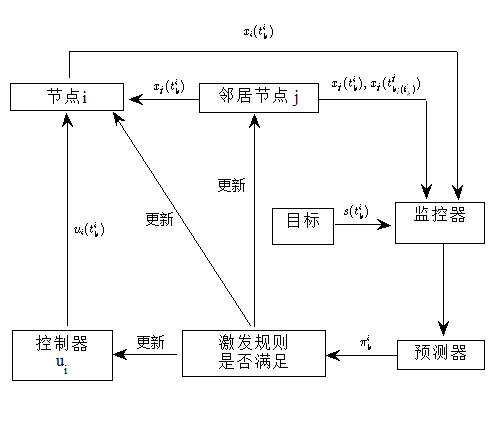
\includegraphics[width=3.2in]{nonlinear/flowchartdec2.png}}
        \end{center}
        \caption{离散监控下的预测激发过程图}\label{flowchart}
        \end{figure}

        与连续监控情形一样, 这里也给出两种不同系统误差上界的激发规则. 不同的是, 离散监控情形下给出的是与系统误差和同步误差相关函数.

        情形c: 基于同步误差上界的离散监控激发规则(简称为DRS激发规则):
        \begin{align}\label{drule:1}
            \nonumber \pi^{i}_{k}=&\max\Big\{t:
            \sum^N_{j=1,j\neq i}(-l_{ij}(r_{t+t^i_k}))\varphi(t,\xi^i_k,\zeta^j_{k_j(t+t^i_k)},x_i(t^i_k),x_j(t^i_k))\\
             &\quad+\tau d_i(r_{t+t^i_k})\varphi(t,\xi^i_k,0,x_i(t^i_k),s(t^i_k))
            \leq\omega \psi(t,\xi^i_k,0,x_i(t^i_k),s(t^i_k))\Big\},\\
           \nonumber t_{k+1}^i&=t_{k}^i+\pi^{i}_{k},
            \end{align}
        其中$\omega=\frac{2\xi\underline{\varepsilon}-\delta\bar{\varepsilon}}{2c\bar{\varepsilon}}$, $0<\delta\leq\frac{2\xi\underline{\varepsilon}}{\bar{\varepsilon}}$, $\xi^i_k=z_i(r_t,t^i_k)$, $\zeta^j_{k_j(t+t^i_k)}=z_j(r_t,t^j_{k_j(t+t^i_k)})$, 函数$z_i(\cdot,\cdot)$, $z_j(\cdot,\cdot)$, $\varphi(\cdot,\cdot,\cdot,\cdot,\cdot)$和$\psi(\cdot,\cdot,\cdot,\cdot,\cdot)$的具体定义将会在\autoref{thm:qn} 中给出.

        情形d: 基于指数函数上界的离散监控激发规则(简称为DRE激发规则):
        \begin{align}\label{drule:2}
             \nonumber \pi^{i}_{k}=&\max\Big\{t:
            \sum^N_{j=1,j\neq i}(-l_{ij}(r_{t+t^i_k}))\mathrm{E}\varphi(t,\xi^i_k,\zeta^j_{k_j(t+t^i_k)},x_i(t^i_k),x_j(t^i_k))\\
            &\quad+\tau d_i(r_{t+t^i_k})\mathrm{E}\varphi(t,\xi^i_k,0,x_i(t^i_k),s(t^i_k))
            \leq ae^{-b(t+t^i_k)}\Big\},\\
            \nonumber t_{k+1}^i&=t_{k}^i+\pi^{i}_{k},
            \end{align}
        其中$a$和$b$是正数.
        \begin{rem}
            离散监控下的激发规则分为两个部分, 一个是预测部分, 另一个是判断部分. 预测部分是整个激发规则最主要部分. 相比于连续的监控激发规则, 离散监控激发规则具有更大计算复杂度.
        \end{rem}
            \begin{algo}[离散监控事件激发算法]\label{algo2}~~

            $1)$ 当$k=0$时, 初始化$t^i_k=0$;

            $2)$ 当$t=t^i_k$时, 控制器收集节点状态信息$x_i(t_k^i), x_j(t^j_{k_j(t_k^i)})$以及$s(t_k^i)$;

            $3)$ 预测机制根据 \eqref{drule:1}$($或者 \eqref{drule:2}$)$预测下一次事件激发间隔$\pi_k^i$;

            $4)$ 当$t_k^i<t<t^i_k+\pi^i_k$时, 如果存在某个邻居节点$j$的事件被激发, 则$t^j_{k_j+1}=t$, 返回$3)$;

            $5)$ 如果$r_t$的状态发生转移, 则返回$2)$;

            $6)$ 当$t=t^i_k+\pi^i_k$时, 则节点$i$的事件被激发, 新的事件激发时刻$t_{k+1}^i=t$. 此时节点$i$以及它的邻居节点和控制器将会更新, 即利用$t^i_{k+1}$时的状态信息替换$t^i_k$时的状态信息, 返回$2)$.
             \end{algo}

        在给出本节定理前, 先证明如下引理:
         \begin{lem}\label{lem:7}
            若函数$f(\cdot): R^n\mapsto R^n$满足$\mathrm{Lipschitz}$条件, 即存在常数$l>0$, 使得对任意$x, y\in R^n$有$\| f(x)-f(y)\|<l\| x-y\|$成立, 则函数$f(\cdot)$ 满足QUAD条件.
        \end{lem}
        \begin{proof}
            取$G=I_n, \Delta=(1+\frac{l}{2})I_n$, 则根据\autoref{lem_leq} 和Lipschitz条件可得
            \begin{align*}
              &\quad(x-y)^\top G[f(x)-f(y)-\Delta(x-y)]\\
              &=(x-y)\top[f(x)-f(y)]-(1+\frac{l^2}{2})(x-y)^\top(x-y)\\
              &\leq\frac{1}{2}(x-y)^\top(x-y)+\frac{1}{2}(f(x)-f(y))^\top(f(x)-f(y))-(1+\frac{l^2}{2})(x-y)^\top(x-y)\\
              &\leq-\frac{1}{2}(1+l^2)(x-y)^\top(x-y)+\frac{l^2}{2}\| x-y\|^2\\
              &=-\frac{1}{2}(x-y)^\top G(x-y).
            \end{align*}
            因此根据\autoref{quad}, 函数$f(\cdot)$满足QUAD条件.
        \end{proof}

        \begin{thm}\label{thm:qn}
            如果假设 $\ref{ass}$ 成立, $f(\cdot)\in L(l_{1},l_{2})$以及$f(\cdot)\in C(\sigma)$, 并且存在正定对角阵$P(u)=\mathrm{diag}\{p_1(u),\cdots,p_N(u)\}$, $u\in S$, 使得对任意$u\in S$, 有
            \begin{align*}
            \bar{\delta}P(u)\otimes G-c\theta\underline{\alpha} P(u)L(u)\otimes G\Gamma
            -c\tau\underline{\alpha} P(u)D(u)\otimes G\Gamma+\frac{1}{2}\sum_{v=1}^{m}q_{uv}P(v)\otimes G\leq 0,
            \end{align*}
            其中$\bar{\delta}=\max_{k}\{\delta_k \}$, $\underline{\alpha}=\min_{k}\{\alpha_{k}\}$,
            那么, 基于$\mathrm{DRS}$激发规则或者$\mathrm{DRE}$激发规则, 按照算法 $\ref{algo2}$, 网络系统 \eqref{sys:init1} 可以实现均方指数同步.
        \end{thm}
        \begin{proof}
        该定理的条件与\autoref{themcon} 的条件是一样的, 唯一不同的是事件激发规则. 因此主要证明思路是考察在离散监控事件激发规则成立的条件下连续监控事件激发规则是否也成立. 这只要判断$\|\tilde{e}_i(t)\|$ 的上界函数和$\|e_i(t)\|$的下界函数是否是$\varphi$和$\psi$即可. 当$l_{ij}(r_t)\neq 0$时, 首先估计$\|(h(x_j(t))-h(x_j(t^i_k)))-(h(x_i(t))-h(x_i(t^i_k)))\|$的上界函数. 显然$h(x_i(\cdot)),h(x_j(\cdot))$满足如下方程:
            \begin{equation}\label{sys:discrete}
                \bigg\{\begin{array}{c}
                    \dot{x}_i(t)=f(x_i(t))+z_i(r_t,t^i_k), \quad    \\
                    \dot{x}_j(t)=f(x_j(t))+z_j(r_t,t^j_{k_j(t)}),
                \end{array}\\
            \end{equation}
       这里$t\in[t^i_k, \min\{ t^i_{k+1}, t^j_{k_j(t)+1}\}]$,
       $z_i(r_t,t^i_k)$和$z_j(r_t,t^i_k)$的定义如下:
        \begin{align}\label{zi}
        \nonumber z_\iota(r_t,t^\iota_k)&=-\theta(t)\rho(t)\sum^N_{j=1}l_{\iota j}(r_{t})\Gamma[h(x_{j}(t_{k}^{\iota}))-h(x_{\iota }(t_{k}^{\iota}))]\\
        &\quad-\tau\rho(t)d_{\iota}(r_{t})\Gamma[h(x_{\iota}(t_{k}^{\iota}))-h(s(t_{k}^{\iota}))].
        \end{align}
        为了讨论的方便, 将方程组 \eqref{sys:discrete} 抽象为一般形式:
            \begin{equation}\label{sys:dis-gener}
                \bigg\{\begin{array}{c}
                    \dot{u}=f(u)+\xi,   \\
                    \dot{v}=f(v)+\zeta,
                \end{array}
            \end{equation}
       其中$u=u(t),v=v(t),u(0)=u_0,v(0)=v_0\in R^n$.
        根据\autoref{ass} 可得
            \begin{align}\label{equ:12}
            \nonumber&\quad\|(h(u)-h(u_0))-(h(v)-h(v_0))\|^2\\
            \nonumber &=\sum^n_{k=1}[ (h_k(u^k)-h_k(u^k_0))-(h_k(v^k)-h_k(v^k_0))]^2\\
            \nonumber &=\sum^n_{k=1}[(h_k(u^k)-h_k(u^k_0))^2+(h_k(v^k)-h_k(v^k_0))^2]\\
            \nonumber &\quad-2\sum^n_{k=1}(h_k(u^k)-h_k(u^k_0))(h_k(v^k)-h_k(v^k_0)) \\
            \nonumber &\leq \bar{\beta}^2\sum^n_{k=1}[ (u^k-u^k_0)^2+(v^k-v^k_0)^2]
            -2\sum^n_{k=1}(h_k(u^k)-h_k(u^k_0))(h_k(v^k)-h_k(v^k_0))\\
            \nonumber &=\bar{\beta}^2\sum^n_{k=1}[(u^k-u^k_0)-(v^k-v^k_0)]^2+\varrho\\
            &=\bar{\beta}^2\|(u-u_0)-(v-v_0)\|^2+\varrho,
            \end{align}
           其中$\bar{\beta}=\max_k\{\beta_k\}$, $\varrho=\sum^n_{k=1}[2\bar{\beta}^2(u^k-u^k_0)(v^k-v^k_0)-2(h_k(u^k)-h_k(u^k_0))(h_k(v^k)-h_k(v^k_0))]$.
            对$\varrho$进一步线性化可得:
            \begin{align}\label{equ:13}
            \nonumber \varrho&\leq\sum^n_{k=1}[2\bar{\beta}^2(u^k-u^k_0)(v^k-v^k_0)+(h_k(u^k)-h_k(u^k_0))^2+(h_k(v^k)-h_k(v^k_0))^2]\\
            \nonumber &\leq\sum^n_{k=1}[2\bar{\beta}^2(u^k-u^k_0)(v^k-v^k_0)+\bar{\beta}^2(u^k-u^k_0)^2+\bar{\beta}^2(v^k-v^k_0)^2]\\
            \nonumber &=\bar{\beta}^2\sum^n_{k=1}(u^k-u^k_0+v^k-v^k_0)^2\\
            &=\bar{\beta}^2\| u-u_0+v-v_0 \|^2.
            \end{align}
        将式 \eqref{equ:13}代入式 \eqref{equ:12}可得
            \begin{align}\label{equ:up1}
            \nonumber &\quad\|(h(u)-h(u_0))-(h(v)-h(v_0))\|^2\\
            &\leq\bar{\beta}^2\|(u-u_0)-(v-v_0)\|^2+\bar{\beta}^2\| u-u_0+v-v_0 \|^2.
            \end{align}
        因为$f(\cdot)$属于函数类$L(l_{1},l_{2})$, 根据方程 \eqref{sys:dis-gener}, 有
            \begin{align}\label{equ:up2}
            \nonumber &\quad\|(u(t)-u_0)-(v(t)-v_0)\|\\
            \nonumber &=\|\int^t_0[f(u(s))-f(v(s))]ds+(\xi-\zeta)t\|\\
            \nonumber &\leq\int^t_0\|f(u(s))-f(v(s))\|ds+\|\xi-\zeta\|t\\
            \nonumber &\leq l_1\int^t_0\|u(s)-v(s)\|ds+|\xi-\zeta\|t\\
             &\leq l_1\int^t_0\|(u(s)-u_0)-(v(s)-v_0)\|ds+(\|\xi-\zeta\|+l_1\|u_0-v_0\|)t.
            \end{align}
        类似地
            \begin{align}\label{equ:up3}
            \nonumber &\quad\| (u(t)-u_0)+(v(t)-v_0)\|\\
            \nonumber &=\|\int^t_0t[f(u(s))+f(v(s))]ds+(\xi+\zeta)t\|\\
            \nonumber &\leq\int^t_0\|f(u(s))+f(v(s))\|ds+\|\xi+\zeta\|t\\
            \nonumber &\leq l_2\int^t_0\|u(s)+v(s)\|ds+\|\xi+\zeta\|t\\
             &\leq l_2\int^t_0\|(u(s)-u_0)+(v(s)-v_0)\|ds+(\|\xi+\zeta\|+l_2\|u_0+v_0\|)t.
            \end{align}
        对式 \eqref{equ:up2} 和式 \eqref{equ:up3} 分别应用Gronwall$-$Bellman不等式, 可得
            \begin{align}\label{equ:up4}
            \|(u(t)-u_0)-(v(t)-v_0)\|\leq\eta_1(\exp^{l_1t}-1),
            \end{align}
       其中$\eta_1=(\|\xi-\zeta\|+l_1\|u_0-v_0\|)/l_1$;
            \begin{align}\label{equ:up5}
            \|(u(t)-u_0)+(v(t)-v_0)\|\leq\eta_2(\exp^{l_2t}-1),
            \end{align}
       其中$\eta_2=(\|\xi+\zeta\|+l_2\|u_0+v_0\|)/l_2$.\\
       结合式 \eqref{equ:up1}、\eqref{equ:up4} 和 \eqref{equ:up5} 可得
            \begin{align}\label{equ:up6}
            \|(h(u)-h(u_0))-(h(v)-h(v_0))\|\leq\varphi(t,\xi,\zeta,u_0,v_0),
            \end{align}
        其中$\varphi(t,\xi,\zeta,u_0,v_0)=\bar{\beta}\sqrt{(\eta_1^2(e^{l_1t}-1)^2+\eta_2^2(e^{l_2t}-1)^2)}$.
        因此$\|(h(u)-h(u_0))-(h(v)-h(v_0))\|$的上界函数已得到.

        接下来估计$\| u(t)-v(t)\|$的下界函数. 根据\autoref{lem_leq} 和方程 \eqref{sys:dis-gener} 可得
            \begin{align}\label{equ:low1}
            \nonumber &\quad\frac{d}{dt}[(u(t)-v(t))^\top(u(t)-v(t))]\\
            \nonumber &=2(u(t)-v(t))^\top(f(u(t))-f(v(t))+\xi-\zeta)\\
            \nonumber &=2(u(t)-v(t))^\top(f(u(t))-f(v(t)))+2(u(t)-v(t))^\top(\xi-\zeta)\\
            \nonumber &\geq 2\sigma(u(t)-v(t))^\top(u(t)-v(t))+2(u(t)-v(t))^\top(\xi-\zeta)\\
            \nonumber &\geq 2\sigma(u(t)-v(t))^\top(u(t)-v(t))-\sigma(u(t)-v(t))^\top(u(t)-v(t))-\frac{1}{\sigma}(\xi-\zeta)^\top(\xi-\zeta)\\
            &=\sigma(u(t)-v(t))^\top(u(t)-v(t))-\frac{1}{\sigma}(\xi-\zeta)^\top(\xi-\zeta).
            \end{align}
        通过利用\autoref{lem:6}, 可以推出
        \begin{align}\label{equ:low3}
        (u(t)-v(t))^\top(u(t)-v(t))\geq (u_0-v_0)^\top(u_0-v_0)e^{\sigma t}-\frac{(\xi-\zeta)^\top(\xi-\zeta)}{\sigma^2}(e^{\sigma t}-1).
        \end{align}
        由于对任意$u_0\neq v_0$,式 \eqref{equ:low3} 右端在小区间$[0, t]$ 上是正数, 故有
        \begin{align}\label{equ:low4}
        \| u(t)-v(t)\|\geq \psi(t,\xi,\zeta,u_0,v_0),
        \end{align}
        其中
        $$\psi(t,\xi,\zeta,u_0,v_0)=\Big\{\| u_0-v_0\|^2 e^{\sigma t}-\frac{\|\xi-\zeta\|^2}{\sigma^2}(e^{\sigma t}-1)\Big\}^\frac{1}{2}.$$

        综上所述, 如果激发规则DRS满足, 那么根据式 \eqref{equ:up6} 和 \eqref{equ:low4}, 激发规则CRS也满足. 类似地, 如果激发规则DRE满足, 那么根据式 \eqref{equ:up6}, 激发规则CRE也满足. 因此根据\autoref{themcon} 的结论, 网络系统 \eqref{sys:init1} 可以实现均方指数同步.
        \end{proof}
        \begin{rem}
        几何上, $\varphi$可以看作是在映射$h$下$u(t)$和$v(t)$从$0$时刻 到$t$时刻的位移差的上界函数, 而$\psi$可以看作是$u(t)$和$v(t)$在$t$ 时刻的距离的下界函数.
        \end{rem}
        \begin{rem}
        在DRS激发规则中, 从$0$时刻到$t$时刻轨道之间的位移差的上界函数被同步误差的下界函数控制, 而在DRE激发规则中, 从$0$时刻到$t$时刻轨道之间的位移差的上界函数被可由参数$a$, $b$调节收敛速度的指数函数控制. 因此DRS激发规则的同步速度比DRE激发规则快, 但DRS激发规则的激发次数比DRE激发规则高. 故在选择激发规则时, 需要在收敛速度和激发次数之间进行取舍. 如果状态监控、数据更新、信号通讯成本较低, 对同步速度要求不高的情况下, 则选用DRE激发规则并选择较大的参数$a$, $b$, 否则选择DRS 激发规则较好.
        四种激发函数的各方面特征比较如下:
        \end{rem}
\begin{table}[!hbp]
\setlength{\abovecaptionskip}{-1pt}
\setlength{\belowcaptionskip}{-1pt}
\caption{四种激发规则的特征比较}\label{table11}
\begin{center}
\begin{tabular}{|c|c|}
\hline
~~~同步速度~~~ & ~~~CRS$>$DRS, CRE$>$DRE~~~\\
\hline
~~~监控成本~~~ & ~~~CRS$=$CRE$>$DRS$>$DRE~~~\\
\hline
~~~计算负荷~~~ & ~~~DRS$>$DRE$>$CRS$>$CRE~~~\\
\hline
~~~激发次数~~~ & ~~~DRS$>$DRE$>$CRS$>$CRE~~~\\
\hline
\end{tabular}
\end{center}
\end{table}
        \begin{rem}
        连续监控激发规则和离散监控激发规则最大的区别在于收集节点状态信息时刻的不同, 在连续监控情形中, 监控器需要不停地监控网络所有节点状态并收集记录其状态信息, 激发规则需要根据收集到数据进行实时更新, 即激发规则每时每刻都需要计算和判断条件是否满足. 而在离散监控激发规则中, 监控器只在事件激发时刻监控节点状态, 当某个节点的事件激发时, 监控器把该节点状态信息传递给预测机制, 预测机制根据收集得到的信息进行预测下一次激发时刻, 即激发规则是需要在激发时刻对数据进行更新.
        \end{rem}
\section{数值模拟}
        本节给出一个数值例子去验证前文提出定理结论的有效性, 并在数值例子中比较四种激发规则的性能. 该例子考虑含有$100$个节点的复杂网络, 每个节点都有$3$个不同的状态组成. 网络模型如下:
        \begin{align}\label{simulate}
        \nonumber\dot{x}_{i}(t)=&f(x_{i}(t))-\theta(t)\rho(t)\sum^{100}_{j=1}l_{ij}(r_{t})\Gamma[h(x_{j}(t_{k}^{i}))-h(x_{i}(t_{k}^{i}))]+u_i(t),\\
         &\quad t_{k}^i\leq t< t_{k+1}^i, \quad i = 1,\cdots,100.\\
        \nonumber u_i(t)=&-\tau \rho(t)d_{i}(r_{t})\Gamma[h(x_{i}(t_{k}^{i}))-h(s(t_{k}^{i}))],
        \end{align}
\begin{figure}[!htb]
\begin{minipage}[t]{0.48\linewidth}
\centering
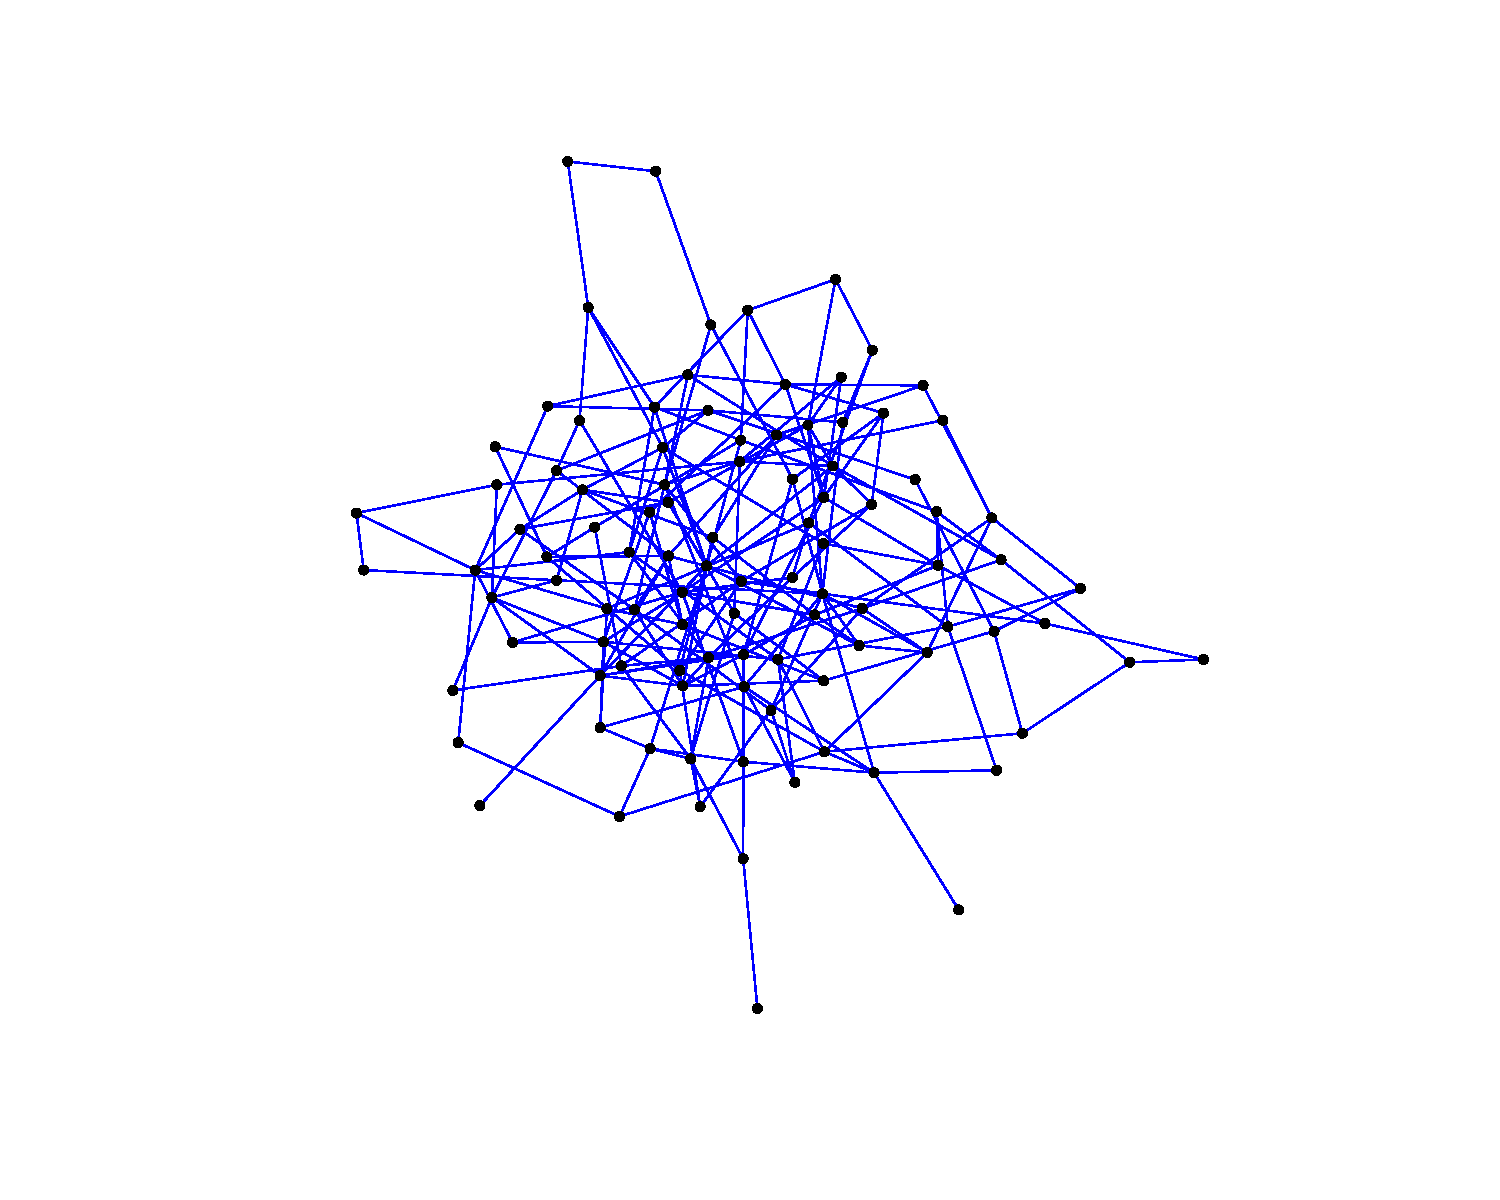
\includegraphics[width=3.2in]{nonlinear/NewL1.pdf}
\caption{马尔可夫链处在状态$1$下的网络拓扑结构.}\label{topology1}
\end{minipage}~~
\begin{minipage}[t]{0.48\linewidth}
\centering
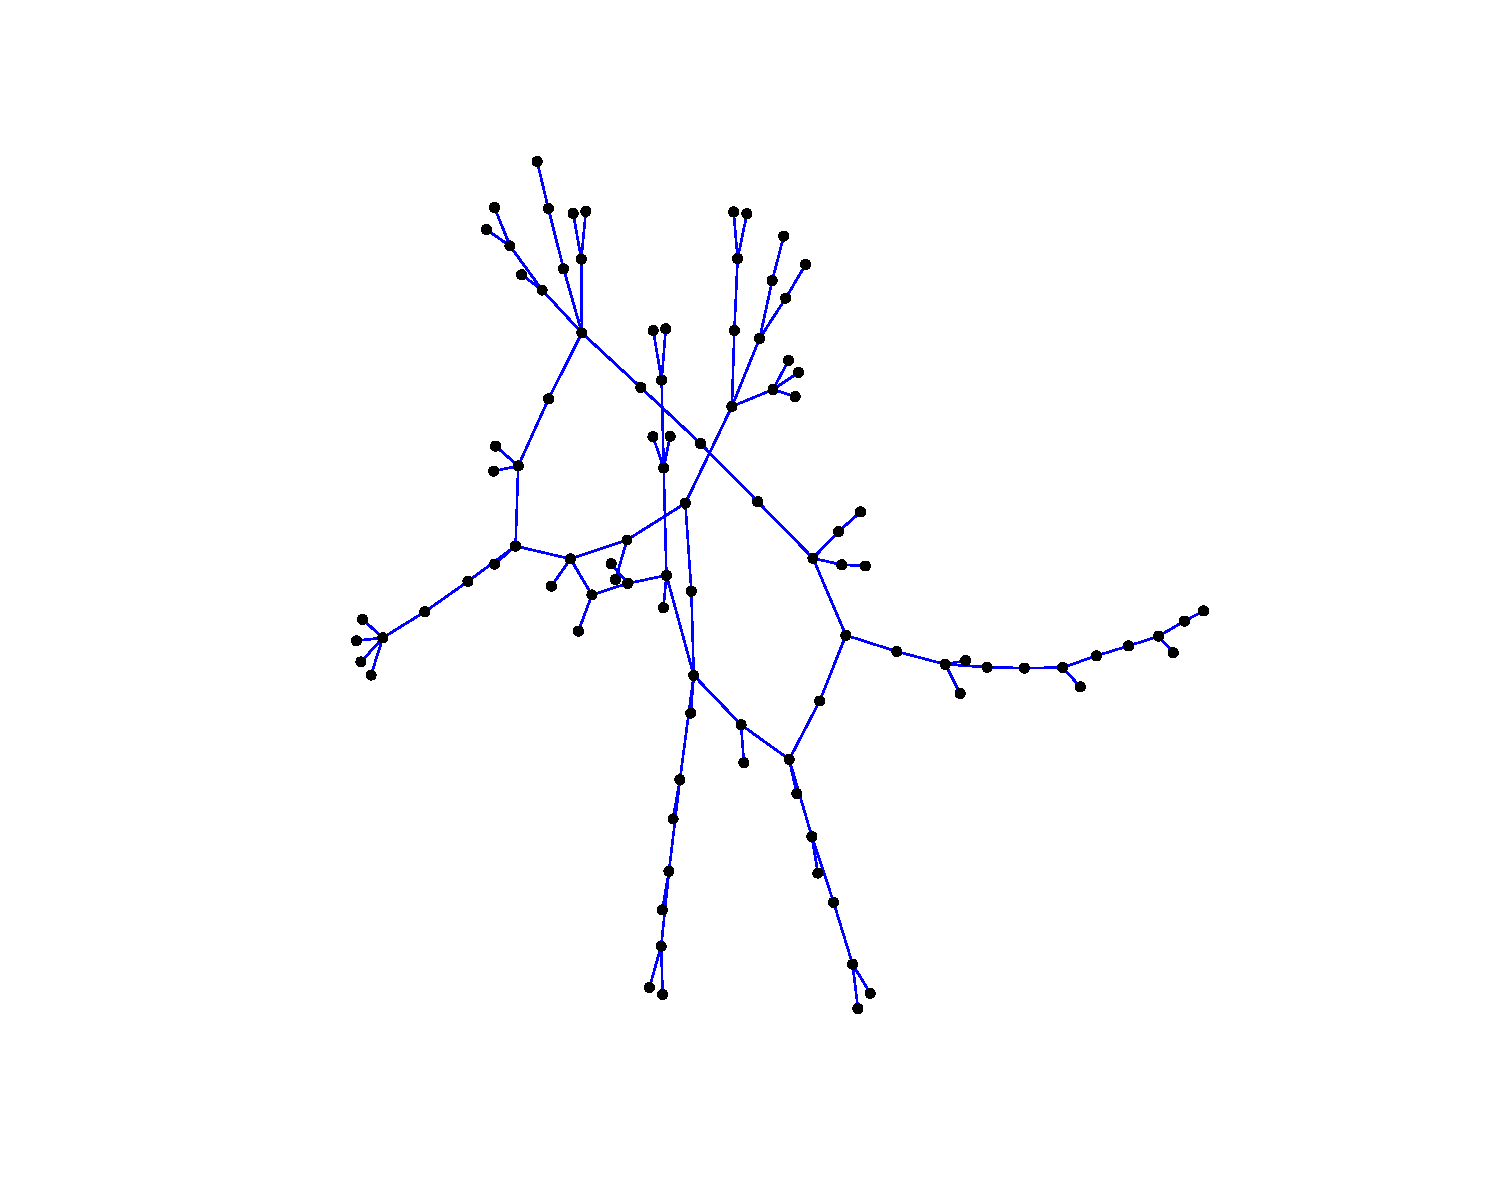
\includegraphics[width=3.2in]{nonlinear/NewL2.pdf}
\caption{马尔可夫链处在状态$2$下的网络拓扑结构.}\label{topology2}
\end{minipage}
\end{figure}
\begin{figure}[!htb]
\begin{minipage}[t]{0.48\linewidth}
\centering
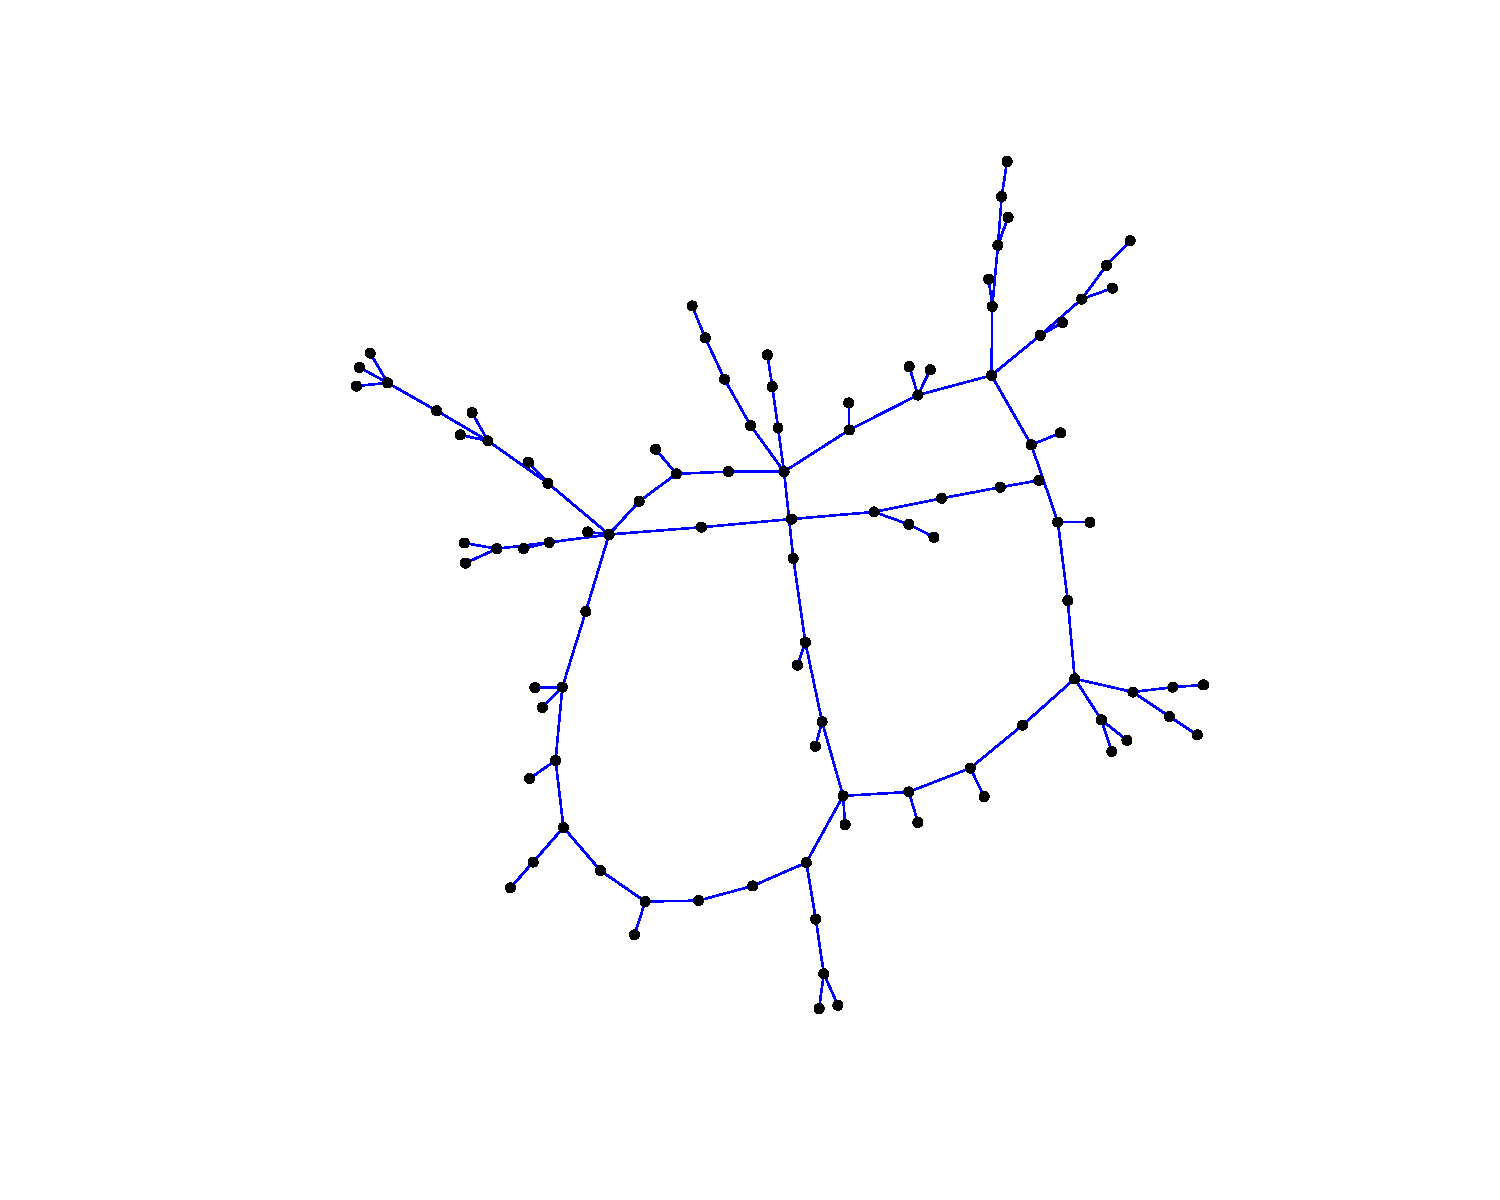
\includegraphics[width=3.2in]{nonlinear/NewL3.pdf}
\caption{马尔可夫链处在状态$3$下的网络拓扑结构.}\label{topology3}
\end{minipage}~~
\begin{minipage}[t]{0.48\linewidth}
\centering
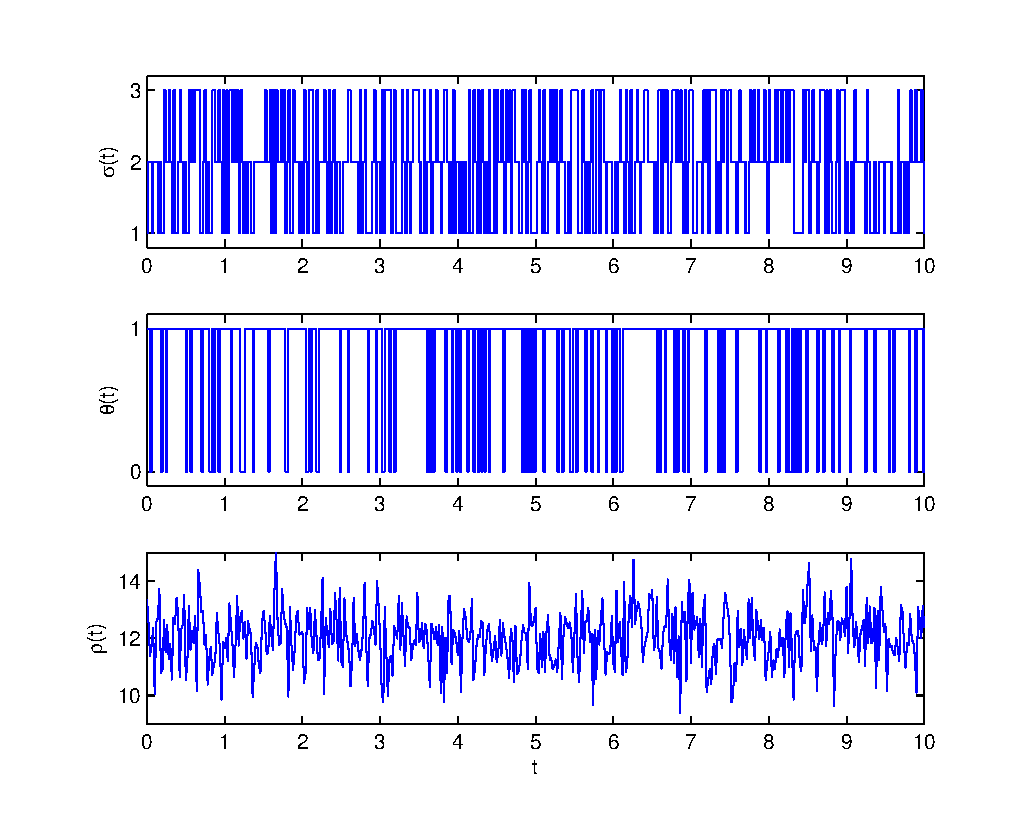
\includegraphics[width=3.2in]{nonlinear/randomvariabel.eps}
\caption{马尔可夫链和随机变量的变化图.}\label{random}
\end{minipage}
\end{figure}
        其中网络可能的拓扑结构见\autoref{topology1}、\autoref{topology2} 和 \autoref{topology3}, 这里选择著名的蔡氏电路系统作为自动力学性态, 它的动力学方程为:
        \begin{align*}
           f(x)=\left(
                  \begin{array}{c}
                    z_1(-x_1+x_2-g(x_1)) \\
                    x_1-x_2+x_3 \\
                    -z_2(x_2) \\
                  \end{array}
                \right)
           \end{align*}
        其中$g(x_1)=r_1x_1+1/2(r_2-r_1)(|x_1+1|-|x_1-1|)$, $z_1=9.78,z_2=14.97,r_1=-0.75,r_2=-1.31$.
        非线性耦合函数以及状态空间为$S=\{1,2,3\}$的马氏链的转移率矩阵如下所示:
           \begin{align*}
           h(x)=\left(
                  \begin{array}{c}
                    2x_1+0.2\sin x_1 \\
                    2x_2+1 \\
                    3x_3+0.5\cos x_3 \\
                  \end{array}
                \right),~~~~
           Q=\left(
            \begin{array}{ccc}
              -8 & 4 & 4 \\
              5 & -8 & 3 \\
              1 & 7 & -8 \\
            \end{array}
          \right).
           \end{align*}
        根据$h(x)$定义, 通过计算可知, 取$\alpha=1.95, \beta=3.25$可是得$h(x)$满足\autoref{ass}. 可能的牵制控制节点为: $\mathcal{D}_1=\{1,20,50,79\}, \mathcal{D}_2=\{1,23,43,54\}$, $\mathcal{D}_3=\{1,4,29,31\}$.
        $\theta(t)$是参数为$p=0.8$伯努利随机变量, $\rho(t)$是参数为$\mu=12,\sigma^2=1$的正态随机变量. 其演变情况如\autoref{random} 所示.
\begin{figure}[!htb]
\begin{minipage}[t]{0.48\linewidth}
\centering
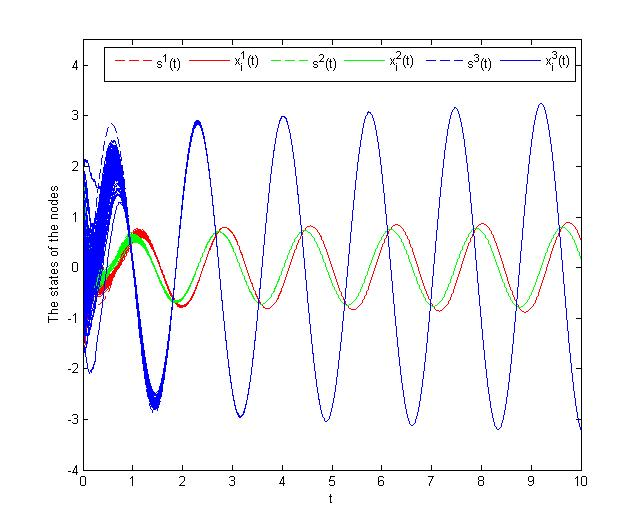
\includegraphics[width=3.2in]{nonlinear/state2223.jpg}
\caption{在连续监控激发规则CRS下, 网络节点状态向量$x^j_i(t)(i=1,2,\cdots,100,j=1,2,3)$和目标轨道$s^j(t)(j=1,2,3)$随时间变化情况.}\label{numcrule1}
\end{minipage}~~
\begin{minipage}[t]{0.48\linewidth}
\centering
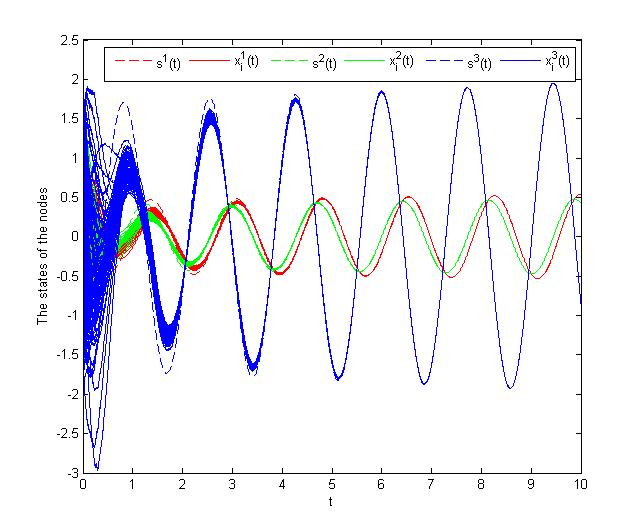
\includegraphics[width=3.2in]{nonlinear/state1612.jpg}
\caption{在连续监控激发规则CRE下, 网络节点状态向量$x^j_i(t)(i=1,2,\cdots,100,j=1,2,3)$和目标轨道$s^j(t)(j=1,2,3)$随时间变化情况.}\label{numcrule2}
\end{minipage}
\end{figure}

\begin{figure}[!htb]
\begin{minipage}[t]{0.48\linewidth}
\centering
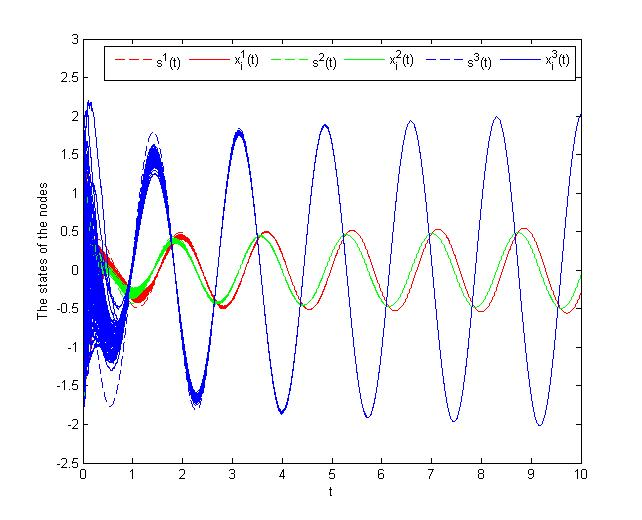
\includegraphics[width=3.2in]{nonlinear/dstateoneand2212.jpg}
\caption{在离散监控激发规则DRS下, 网络节点状态向量$x^j_i(t)(i=1,2,\cdots,100,j=1,2,3)$和目标轨道$s^j(t)(j=1,2,3)$随时间变化情况.}\label{numdrule1}
\end{minipage}~~
\begin{minipage}[t]{0.48\linewidth}
\centering
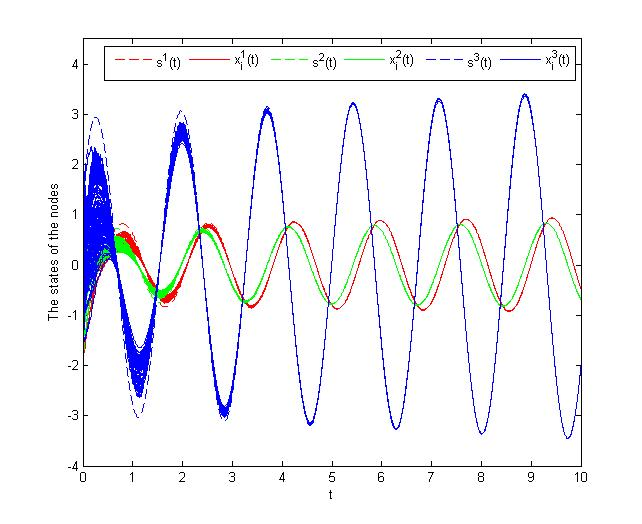
\includegraphics[width=3.2in]{nonlinear/dstatedata3840.jpg}
\caption{在离散监控激发规则DRE下, 网络节点状态向量$x^j_i(t)(i=1,2,\cdots,100,j=1,2,3)$和目标轨道$s^j(t)(j=1,2,3)$随时间变化情况.}\label{numdrule2}
\end{minipage}
\end{figure}

        下面选择相应的参数使得\autoref{themcon} 和\autoref{thm:qn} 的条件成立.
        取$\Gamma=G=P(u)=I_3, \Delta=\epsilon I_3$, $\epsilon=11.7$. 通过对函数$f$求偏导数可得其可能的Jacobin矩阵为:
        \begin{align*}
        \left(
              \begin{array}{ccc}
                3.0318 & 9.78 & 0 \\
                1 & -1 & 1 \\
                0 & -14.97 & 0 \\
              \end{array}
            \right),~~~~
        \left(
              \begin{array}{ccc}
                -2.445 & 9.78 & 0 \\
                1 & -1 & 1 \\
                0 & -14.97 & 0 \\
              \end{array}
            \right).
        \end{align*}
        因此取$\xi=\epsilon-9.1207=2.5793$, 其中$9.1207$是Jacobin矩阵对称部分的最大特征值.
\begin{figure}[!htb]
\begin{minipage}[t]{0.48\linewidth}
\centering
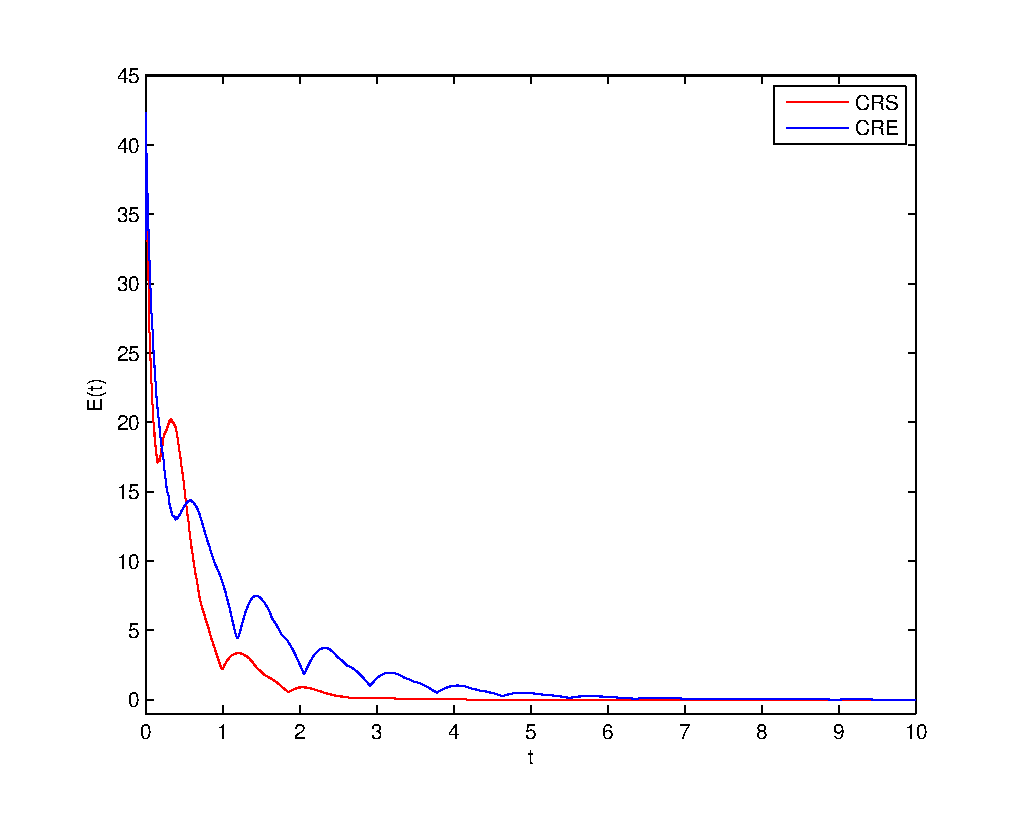
\includegraphics[width=3.2in]{nonlinear/Totallerror1.eps}
\caption{在连续监控激发规则CRS和激发规则CRE下, 网络总误差轨道$E(t)$随时间变化情况.}\label{Totallerror1}
\end{minipage}~~
\begin{minipage}[t]{0.48\linewidth}
\centering
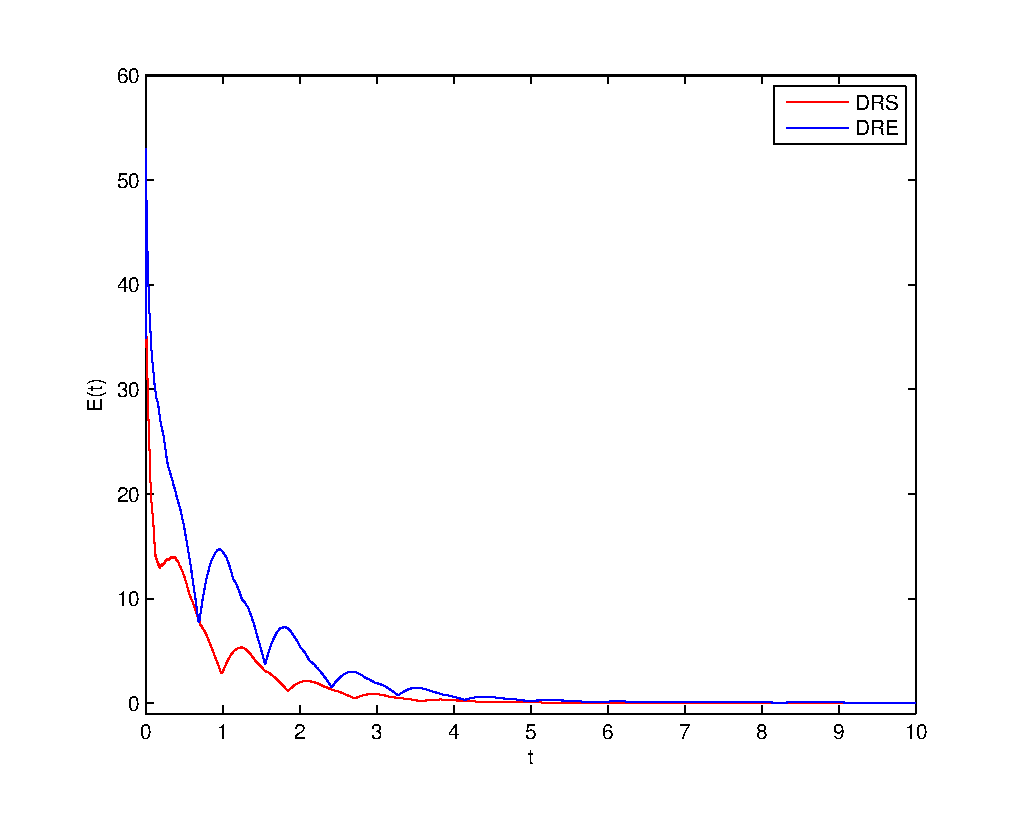
\includegraphics[width=3.2in]{nonlinear/Totallerror2.eps}
\caption{在离散监控激发规则DRS和激发规则DRE下, 网络总误差轨道$E(t)$随时间变化情况.}\label{Totallerror2}
\end{minipage}
\end{figure}
\begin{figure}[!htb]
\begin{minipage}[t]{0.48\linewidth}
\centering
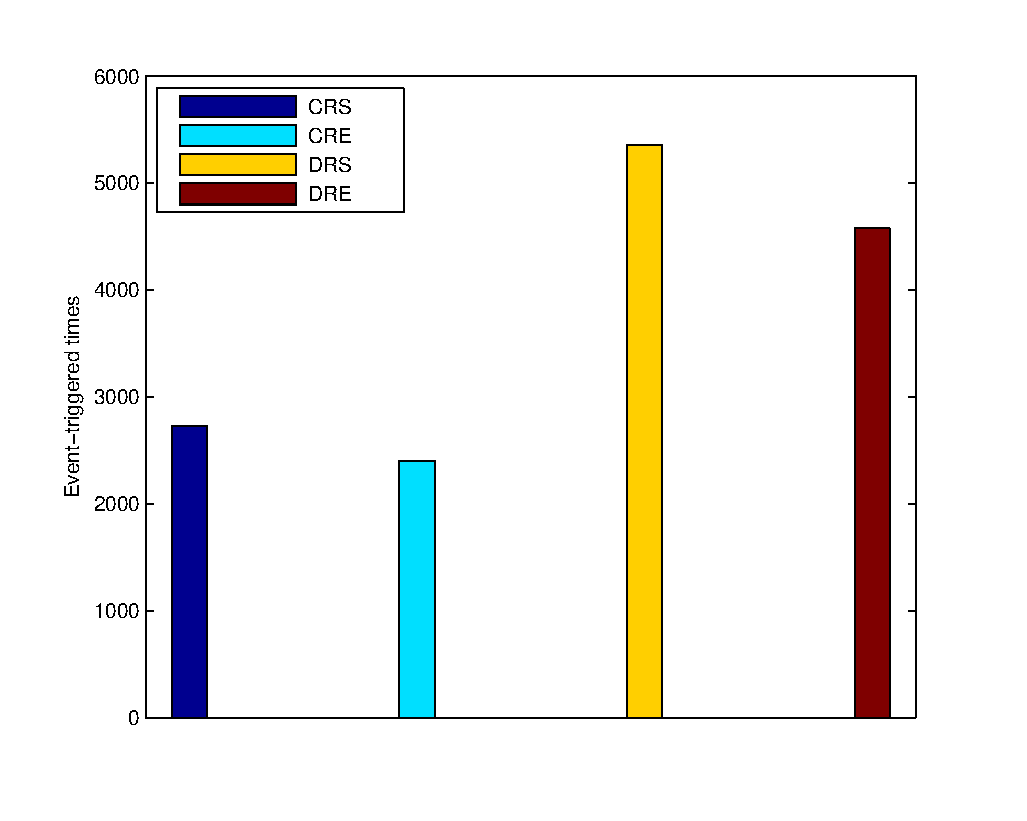
\includegraphics[width=3.2in]{nonlinear/triggertime.eps}
\caption{连续监控和离散监控四种激发规则每个节点平均激发次数.}\label{tritime}
\end{minipage}~~
\begin{minipage}[t]{0.48\linewidth}
\centering
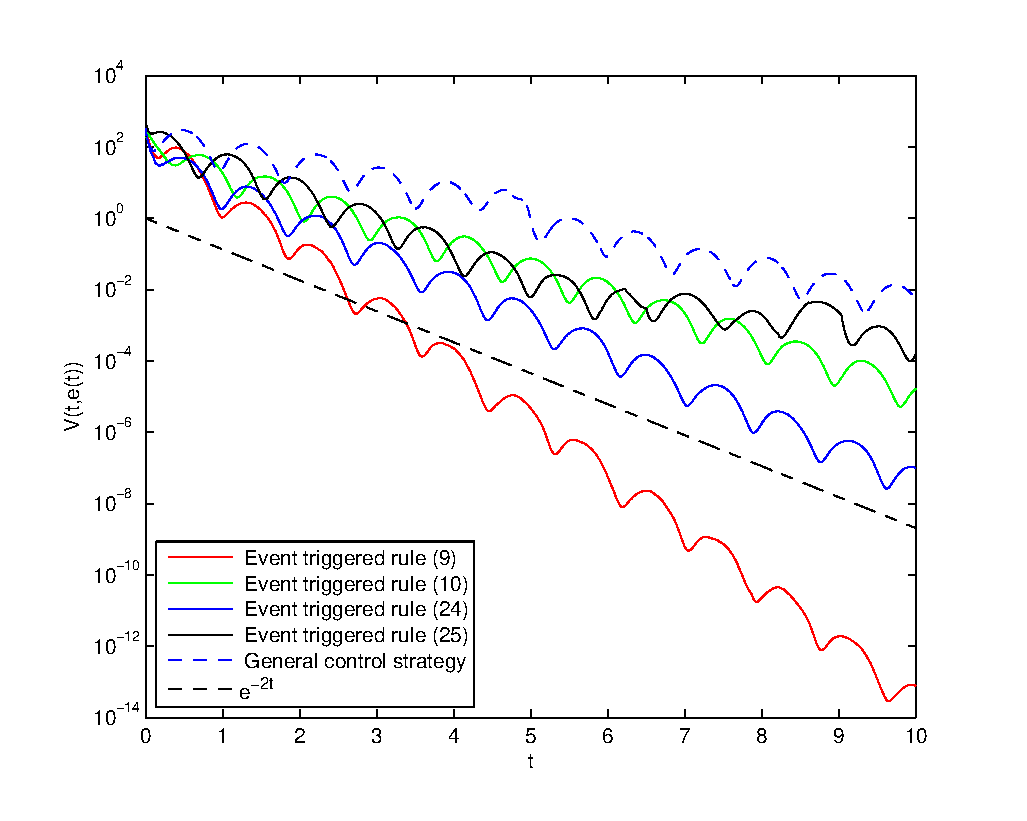
\includegraphics[width=3.2in]{nonlinear/Vt.eps}
\caption{Lyapunov-Krasovskii函数$V(t)$.}\label{Vt}
\end{minipage}
\end{figure}
        接下来估计参数$l_1,l_2$, 根据微分中值定理可得:
        \begin{align*}
        \quad(f(u)f(v))^\top((f(u)-f(v)))
        &=(J(\varsigma)(u-v))^\top(J(\varsigma)(u-v))\\
        &=(u-v)^\top J(\varsigma)^\top J(\varsigma)(u-v)\\
        &\leq\lambda_{max}(J(\varsigma)^\top J(\varsigma))(u-v)^\top(u-v)\\
        &\leq17.9826^2(u-v)^\top(u-v)
        \end{align*}
        故取$l_1=17.9826$可使得$\parallel f(u)-f(v)\parallel\leq l_1\parallel u-v\parallel$. 记$\nu=z_1(1+r_1)$或者$z_1(1+r_2)$, $\mu=x+s$, 于是
        \begin{align*}
         &\quad\| f(x)+f(s)\|^2\\
         &=(-\nu\mu_1+z_1)^2+(\mu_1-\mu_2+\mu_3)^2+(z_2\mu_2)^2\\
         &=(\nu^2+1)\mu_1^2+(z_1^2+z_2^2+1)\mu_2^2+\mu_3^2-2(z_1\nu+1)\mu_1\mu_2+2\mu_1\mu_3-2\mu_2\mu_3\\
         &\leq(\nu^2+z_1\nu+3)\mu_1^2+(z_1^2+z_2^2+z_1\nu+3)\mu_2^2+3\mu_3^2\\
         &\leq32.8901\mu_1^2+346.6614\mu_2^2+3\mu_3^2\\
         &\leq18.6188^2\| x+s\|^2.
        \end{align*}
\begin{figure}[!htb]
\begin{minipage}[t]{0.48\linewidth}
\centering
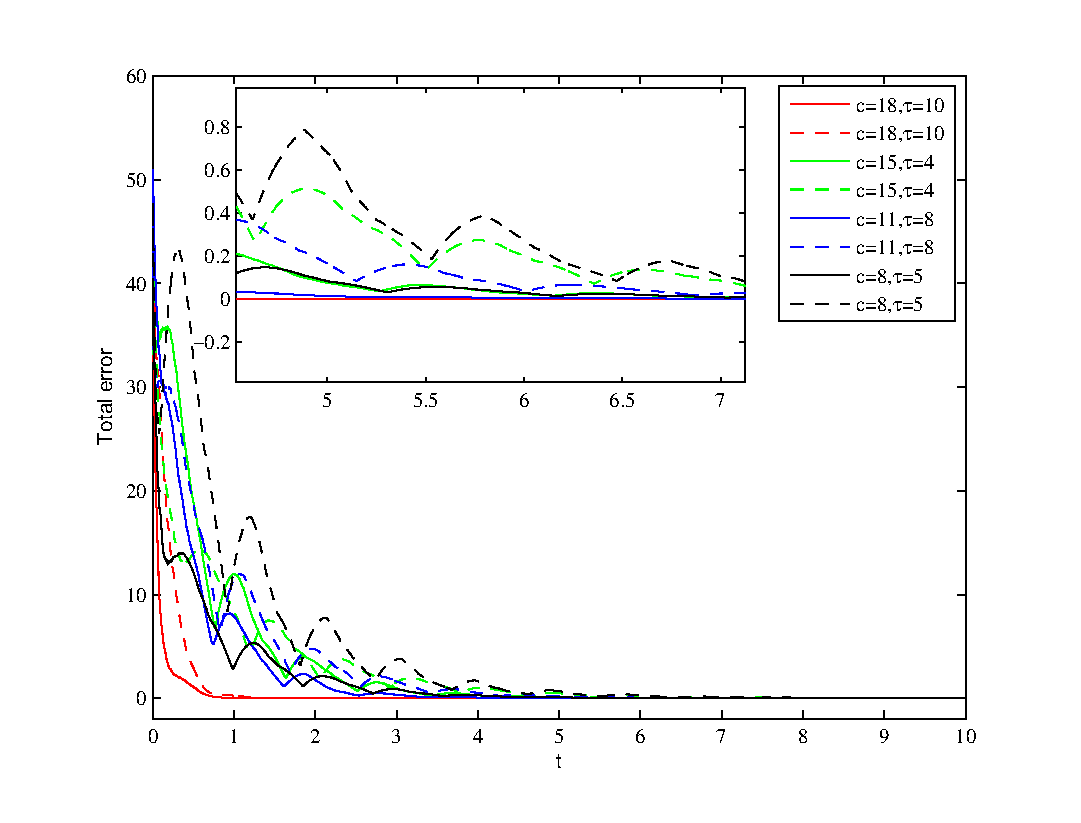
\includegraphics[width=3.2in]{nonlinear/diffstrength.eps}
\caption{连续监控下不同耦合强度和控制强度的系统总误差图, 其中实线表示CRS 激发规则, 虚线表示CRE激发规则.}\label{cdiffstrength}
\end{minipage}~~
\begin{minipage}[t]{0.48\linewidth}
\centering
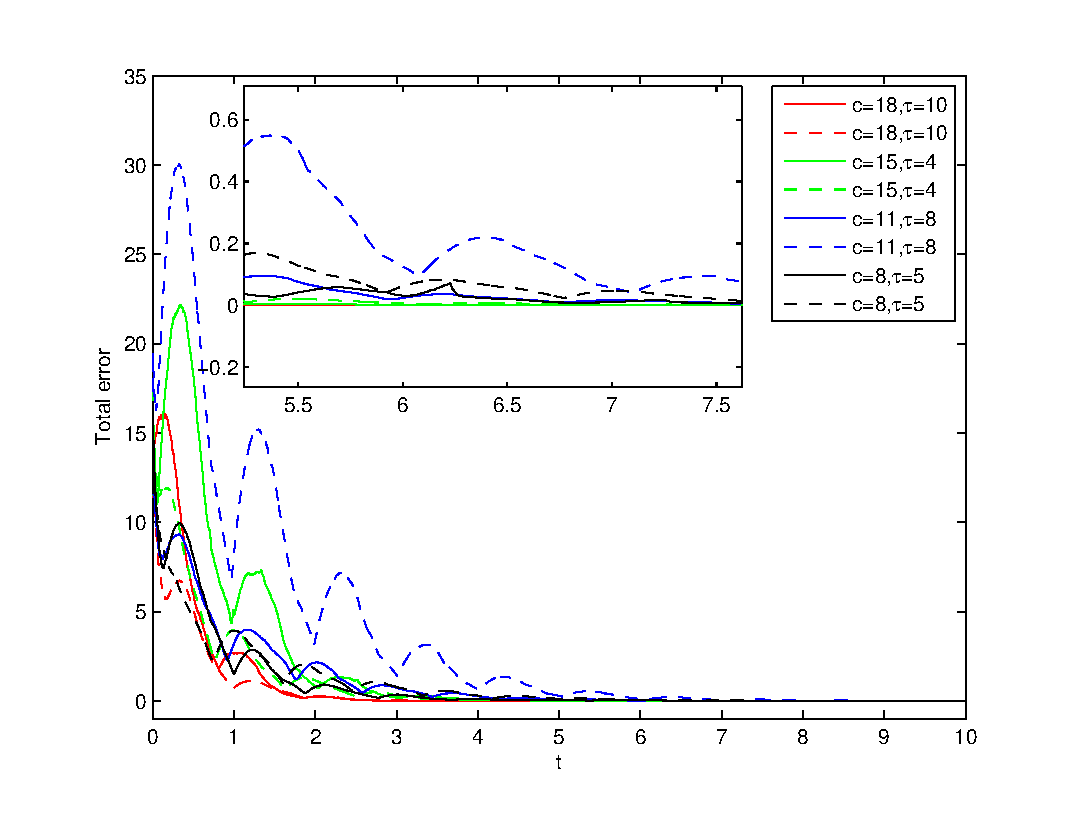
\includegraphics[width=3.2in]{nonlinear/differentstength.eps}
\caption{离散监控下不同耦合强度和控制强度的系统总误差图, 其中实线表示DRS 激发规则, 虚线表示DRE激发规则.}\label{ddiffstrength}
\end{minipage}
\end{figure}
       因此取$l_2=18.6188$, 可使得$\| f(x)+f(s)\|\leq l_2\| x+s\|$. 综上所述, $f(\cdot)$属于函数类$L(l_1,l_2)$.

        选取$c=12, \theta=0.8, \tau=2.8$, 那么对所有$u\in S$, $\epsilon I-c\theta\alpha L(u)-c\alpha\tau D(u)<0$. 即\autoref{themcon} 和\autoref{thm:qn} 的条件成立. 取$\delta=0.05$, $a=b=0.2$, 通过计算可得$\omega=0.2$.

        利用欧拉法, 取步长为$0.01$, 区间为$[0,10]$. 通过MATLAB求解微分方程 \eqref{simulate} 并画出相应的变化图, 见\autoref{numcrule1} 至\autoref{ddiffstrength}.

        \autoref{numcrule1} 至\autoref{numdrule2} 展示了在四种激发规则下, 节点状态向量轨道$x^j_i(t)(i=1,2,\cdots,100,j=1,2,3)$的变化情况. 从图中可以看出, 所有节点的状态都趋于同步. 因此本文提出的激发规则是有效的.

        为了更好的比较四种激发规则的性能, 下面画出不同激发规则下的网络系统总同步误差, 其定义为如下:
        $$E(t)=\sqrt{\sum_{i=1}^{100}\sum_{j=1}^3(x_i^j(t)-s^j(t))^2}. $$

        \autoref{Totallerror1} 和\autoref{Totallerror2} 描述了在四种激发规则下网络系统总误差随时间变化过程, 从这两个图可以看出, 系统误差都能够趋于零. 但各种激发规则趋于零的时间有稍微的差别. CRS激发规则达到同步所需要的时间比CRE要快一些. DRS激发规则达到同步所需要的时间比DRE要快一些. 即基于误差上界的激发规则有较短的同步时间. 这与\autoref{table11} 分析的结果一致.


        \autoref{tritime} 和 \autoref{Vt} 分别是四种激发规则的平均激发次数和Lyapunov—Krasovskii函数$V(t)$. 从图中看出, 离散监控的激发规则的平均激发次数要高于连续情形, 四种事件激发函数的平均激发次数从高到低依次是: DRS$>$DRE$>$CRS$>$CRE, 即要使得同步时间较快则需要付出更高的激发次数. 四种激发规则的$V(t)$ 收敛速度都比$e^{-2t}$快, 即网络能够实现指数同步. \autoref{cdiffstrength} 和\autoref{ddiffstrength} 是选择几个不同耦合强度和控制强度时的系统误差图, 图中可以看出, 复杂网络节点间耦合强度和输入的控制强度越大, 系统获得同步所需要的时间就越短.

\section{小结}
    在这一章节, 主要研究了一类带有马氏切换非线性耦合的时滞网络, 主要引进了事件激发采样的牵制控制策略. 分析了连续和离散两种情形下的基于不同误差上界的激发规则, 利用Lyapunov—Krasovskii稳定性理论和Kronecker积的性质推导了充分的均方指数同步条件, 并在数值模拟中比较了四种不同激发规则之间的同步性能以及消耗的成本.
